\documentclass{article}

\usepackage{geometry}
\geometry{letterpaper, total={7in, 10in} }
\usepackage{booktabs}
\usepackage{graphicx}
\usepackage{verbatim}

\title{CSCI 4360 Data Science II \protect\\ Project II}
\author{Ayush Kumar, Brandon Amirouche, Faisal Hossain}
\date{March 30, 2021}

\begin{document} 
	
	\maketitle
	\tableofcontents
	\newpage
	
	\section{AutoMPG}
	
	The Goal of the AutoMPG Dataset is to predict the Miles per Gallon that a car will have 
	based on a few key characteristics. 
	
	\begin{enumerate}
		\item cylinders 
		\item displacement 
		\item horsepower 
		\item weight 
		\item acceleration 
		\item model-year
	\end{enumerate}

	\subsection{Results}

	We want to find out if using feed-forward neural networks will offer some sort of advantage over 
	traditional regression modeling. The AutoMPG Dataset only has a few observations so it is highly 
	unlikely that we will be able to fully leverage the power of neural networks because our dataset 
	isn't large enough to have such complicated patterns hidden in it. In addition to this, neural networks 
	are computationally expensive and require much more hyper parameter tuning than a traditional or 
	transformed regression model. The following table summarizes the results of our findings in terms 
	of $R^2$, $\bar R^2$ $R^2_{cv}$ and $AIC$ for some traditional regression models, and some neural networks. 
	

	\begin{tabular}{|c|c|c|}
		\hline
		& $R^2$ & $\bar R^2$ \\ \hline
		Multiple Linear Regression            & 0.807 & 0.806      \\ \hline
		Quadratic Regression                  & 0.876 & 0.873      \\ \hline
		Quadratic Regression with Cross Terms & 0.883 & 0.873      \\ \hline
		Transformed Regression                & 0.851 & 0.848      \\ \hline
		Perceptron                            & 0.734 & 0.704      \\ \hline
		3 Layer Neural Network                & 0.793 & 0.790      \\ \hline
		4 Layer Neural Network                & 0.778 & 0.776      \\ \hline
	\end{tabular}

	As the directly comparable results show (some results were not stable between python and scala) we can see that the neural 
	network models offer little to no benefit in comparison to the traditional regression models. In fact 
	while the 3 and 4 layer networks perform quite well, they still lag behind a simple quadratic regression, and 
	oftentimes are not stable over repeated training loops. The 4-Layer network is especially prone to breaking, but 
	this may be because of the small size of the dataset in comparison to the number of parameters. 
	
	\subsection{Variable Selection}
	
	Forward Selection, Backward Elimination, and Stepwise Regression for the 4 models. Some turned out to be 
	not be very stable because of the randomness associated with neural networks. Nonetheless we have some results in the following graphs. 
	
	Perceptron Selection Process (Forward, Backward, Stepwise)
	
	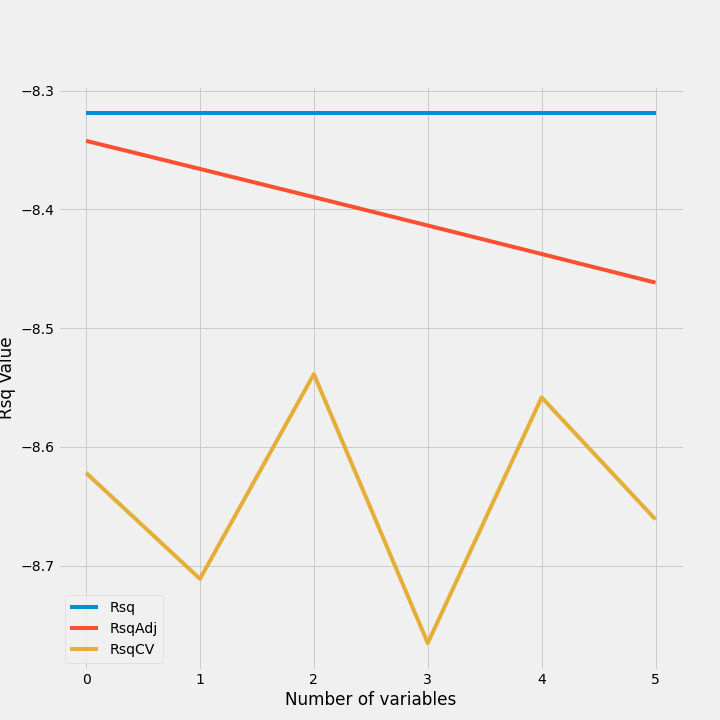
\includegraphics[scale = 0.2]{../plots/python/AutoForwardPCP.png} 
	\includegraphics[scale = 0.2]{../plots/python/BackwardPCP.png}
	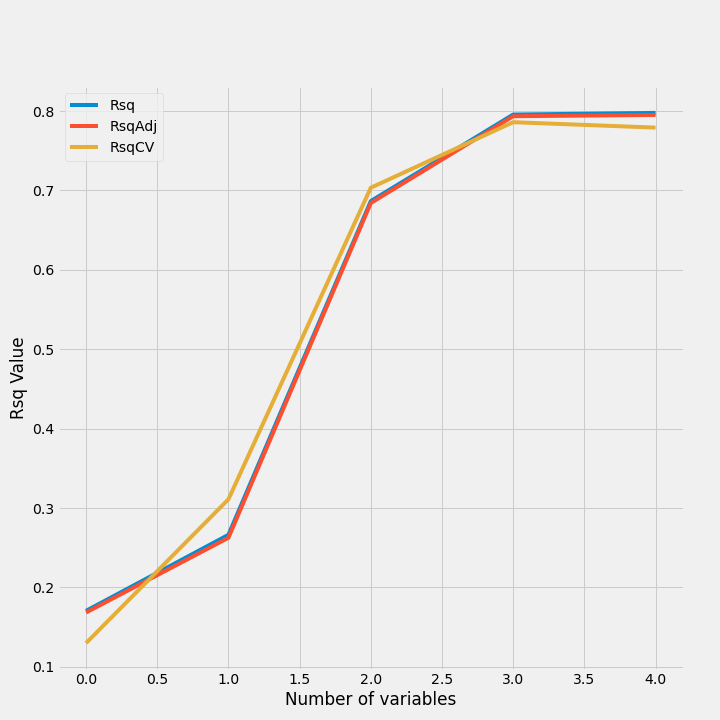
\includegraphics[scale = 0.2]{../plots/python/StepwisePCP.png}
	
	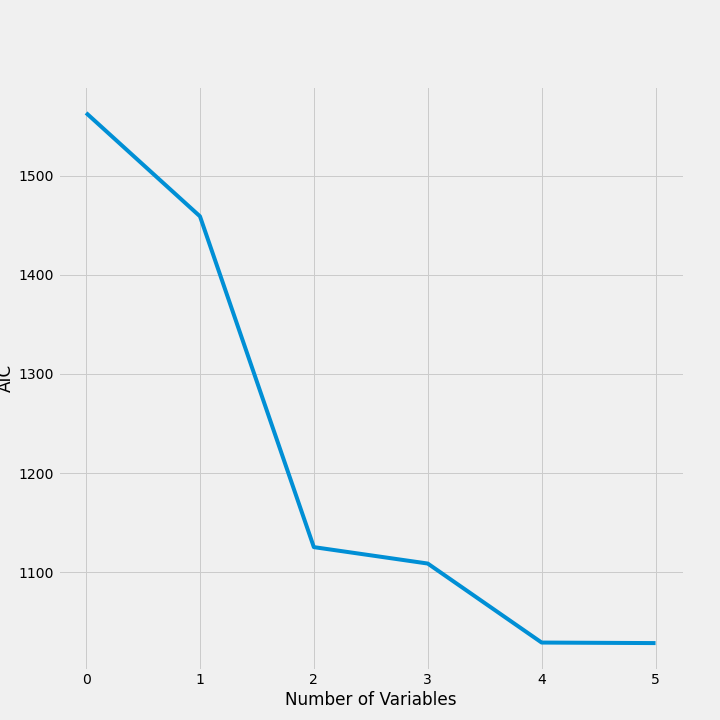
\includegraphics[scale = 0.2]{../plots/python/AICAutoForwardPCP.png} 
	\includegraphics[scale = 0.2]{../plots/python/AICBackwardPCP.png}
	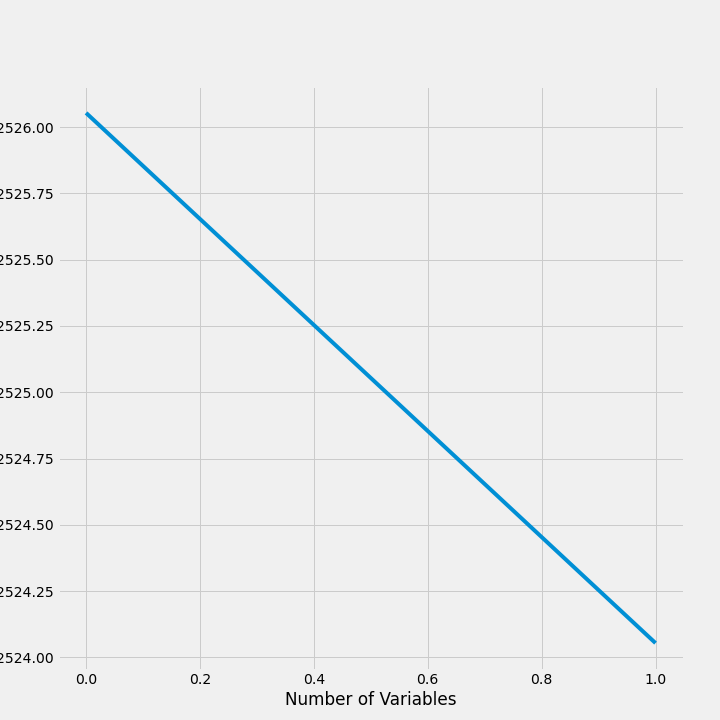
\includegraphics[scale = 0.2]{../plots/python/AICStepwisePCP.png}
	
	3 Layer Network Selection Process (Forward, Backward, Stepwise)
	
	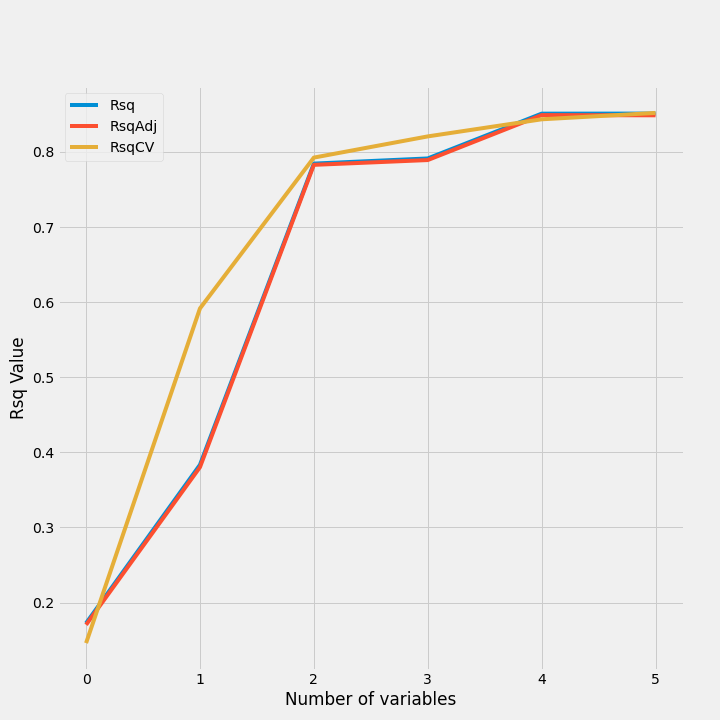
\includegraphics[scale = 0.2]{../plots/python/AutoForward3L.png} 
	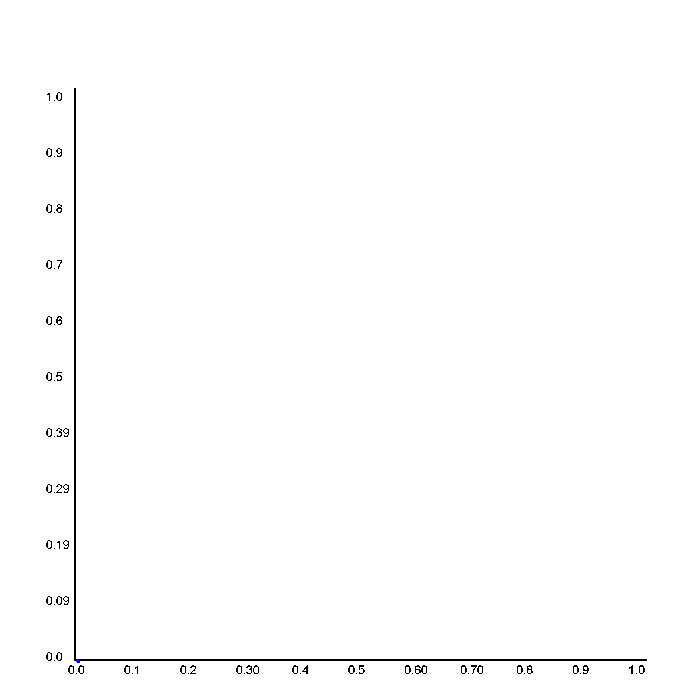
\includegraphics[scale = 0.2]{../plots/python/Backward3L.png}
	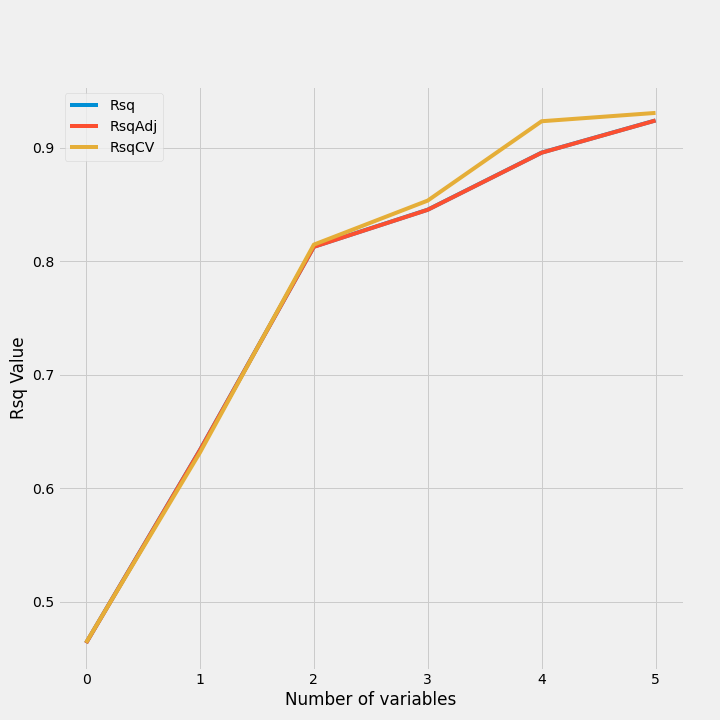
\includegraphics[scale = 0.2]{../plots/python/Stepwise3L.png}
	
	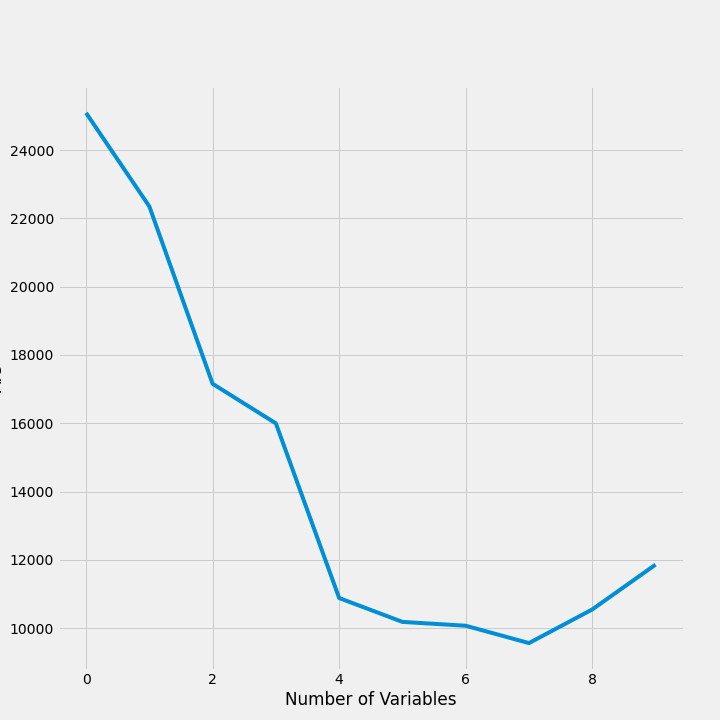
\includegraphics[scale = 0.2]{../plots/python/AICAutoForward3L.png} 
	\includegraphics[scale = 0.2]{../plots/python/AICBackward3L.png}
	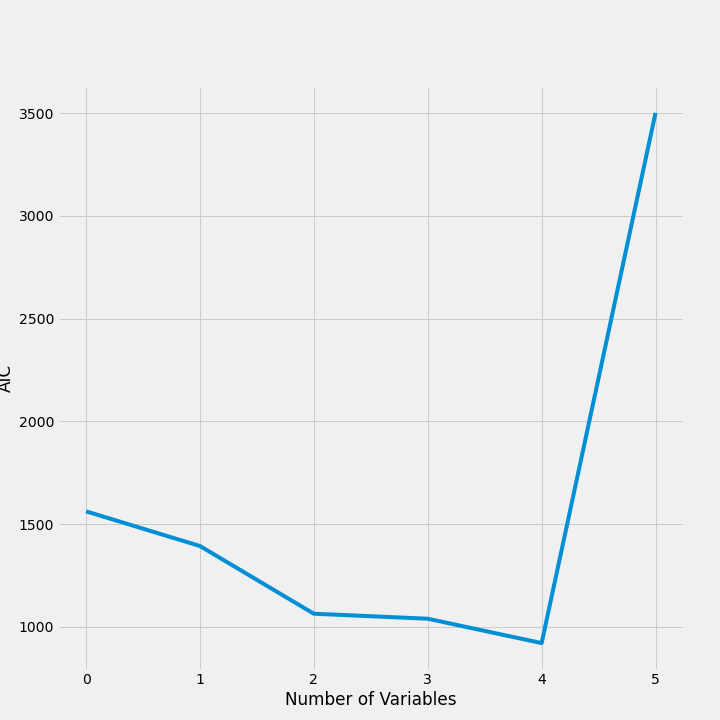
\includegraphics[scale = 0.2]{../plots/python/AICStepwise3L.png}
	
	4 Layer Network Selection Process (Forward, Backward, Stepwise)
	
	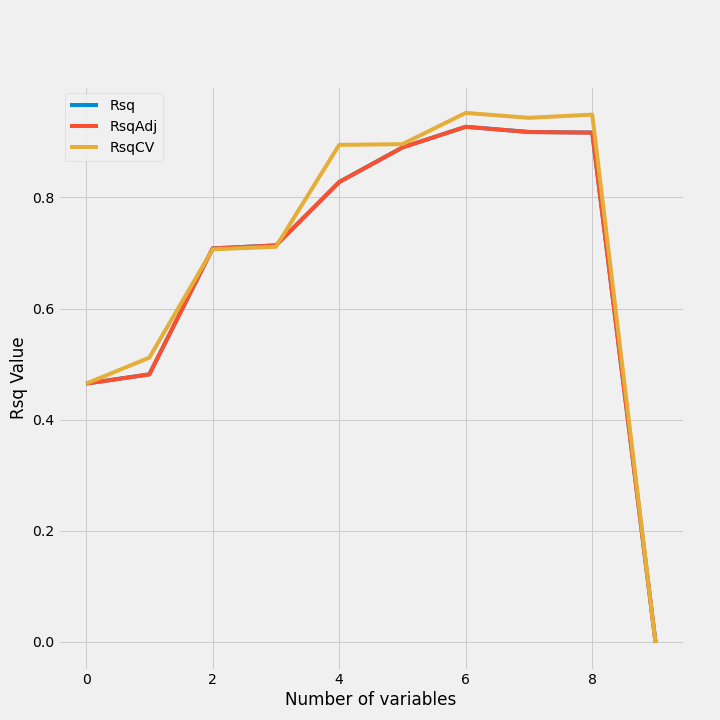
\includegraphics[scale = 0.2]{../plots/python/AutoForward4L.png} 
	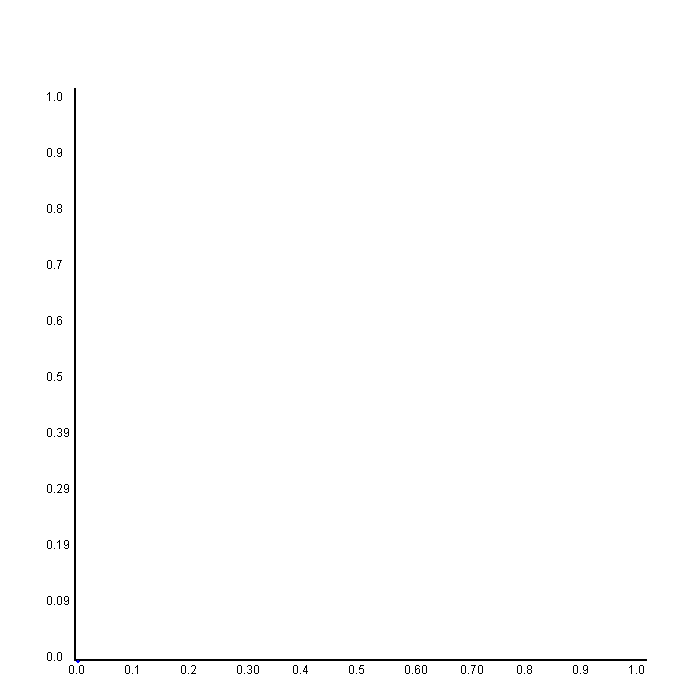
\includegraphics[scale = 0.2]{../plots/python/Backward4L.png}
	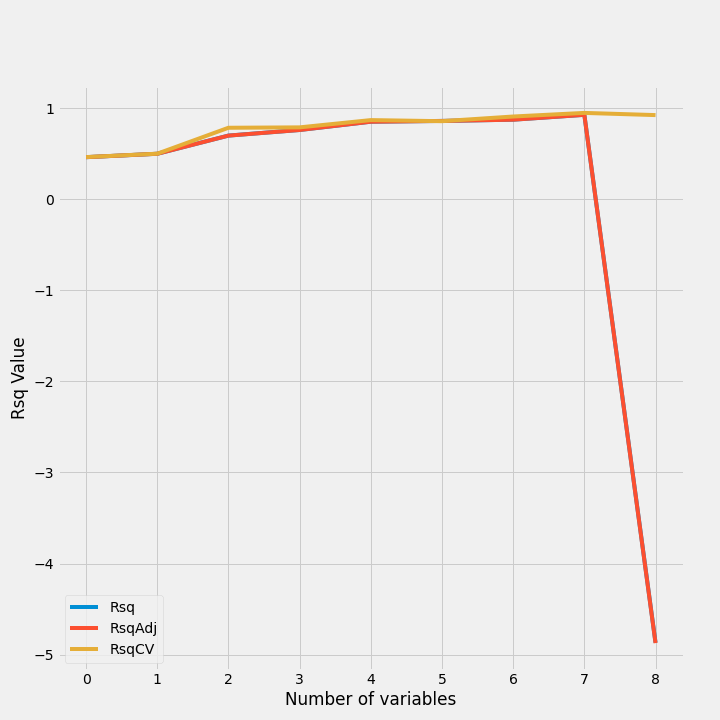
\includegraphics[scale = 0.2]{../plots/python/Stepwise4L.png}
	
	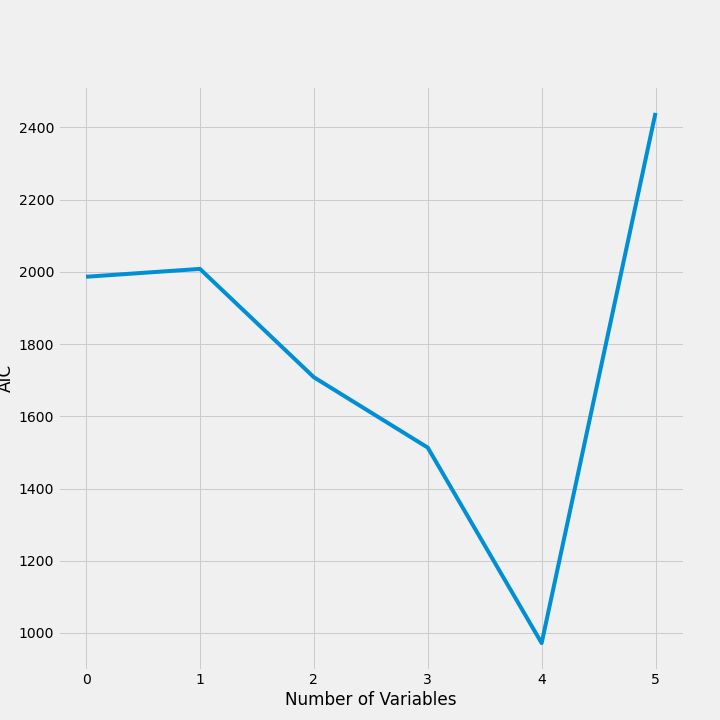
\includegraphics[scale = 0.2]{../plots/python/AICAutoForward4L.png} 
	\includegraphics[scale = 0.2]{../plots/python/AICBackward4L.png}
	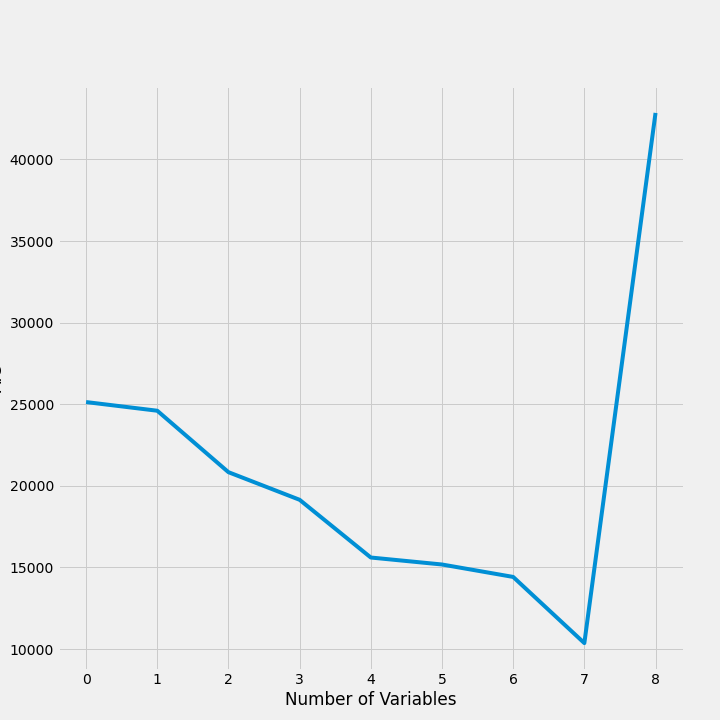
\includegraphics[scale = 0.2]{../plots/python/AICStepwise4L.png}
	
	As can be seen here is some very peculiar behavior with the model 
	occasionally failing to converge. 
	
	
\end{document}